\label{chapter:A-2-Estimaciones Para Open Fing}

\section{Proceso}
\label{section:Proceso}
\label{Proceso}
En esta sección se detallan los distintos procesos necesarios para pasar los videos de OpenFing a vectores en la base vectorial que utiliza el chatbot.

\subsection[Scraping de OpenFing]{Scraping de OpenFing}
\label{Scraping de OpenFing}
Se comienza haciendo \textit{scraping} de OpenFing. De cada clase interesa:
\begin{itemize}
    \item el enlace específico al video, típicamente en servidores de OpenFing y con extensión mp4;
    \item el curso del que proviene la clase, identificado por el acrónimo ya asignado por OpenFing;
    \item el número de la clase, que también figura en OpenFing;
    \item el curso relacionado, que es el curso de la lista de la página inicial por el cual se llegó a esa clase. El curso relacionado puede coincidir con el propio curso.
\end{itemize}
Todos estos datos constituyen los metadatos.

\begin{figure}[htbp]
    \centering
    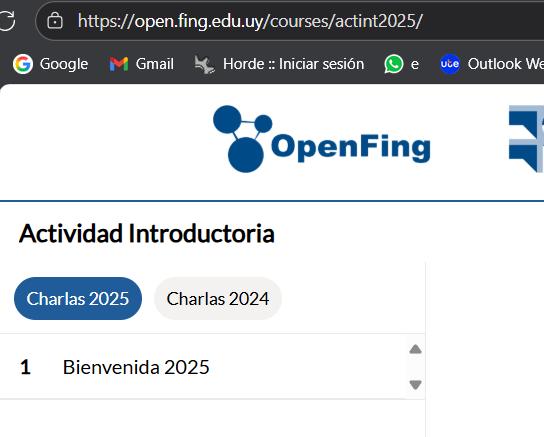
\includegraphics[width=0.8\textwidth]{Nuestro/Imagenes/EstimacionesOpenFing/ActIntroductoria_acronimo}
    \caption{Captura de pantalla de Actividad Introductoria 2025 \protect\footnote{\url{https://open.fing.edu.uy/courses/actint2025/}}.}
    \label{fig:estimaciones-acronimo}
\end{figure}

Por ejemplo, la clase ``Bienvenida 2025'' tiene los siguientes datos: curso \textit{actint2025} (por la URL), número 1 y curso relacionado \textit{actint2025}. Las clases de ``Charlas 2024'' tienen como curso relacionado \textit{actint2025}, ya que para acceder a ellas es necesario pasar primero por el curso de Actividad Introductoria.

Lo que se hizo concretamente fue recorrer cada uno de los cursos de la pantalla inicial de OpenFing, es decir, todas las clases de los cursos que aparecen en la pantalla inicial o que son referenciados por alguno de estos. Hay cursos publicados que no están en esa lista ni son referenciados por ninguno de ellos, así como clases que no están publicadas. Esas clases no se pudieron contabilizar porque no se puede acceder a ellas.

\begin{figure}[htbp]
    \centering
    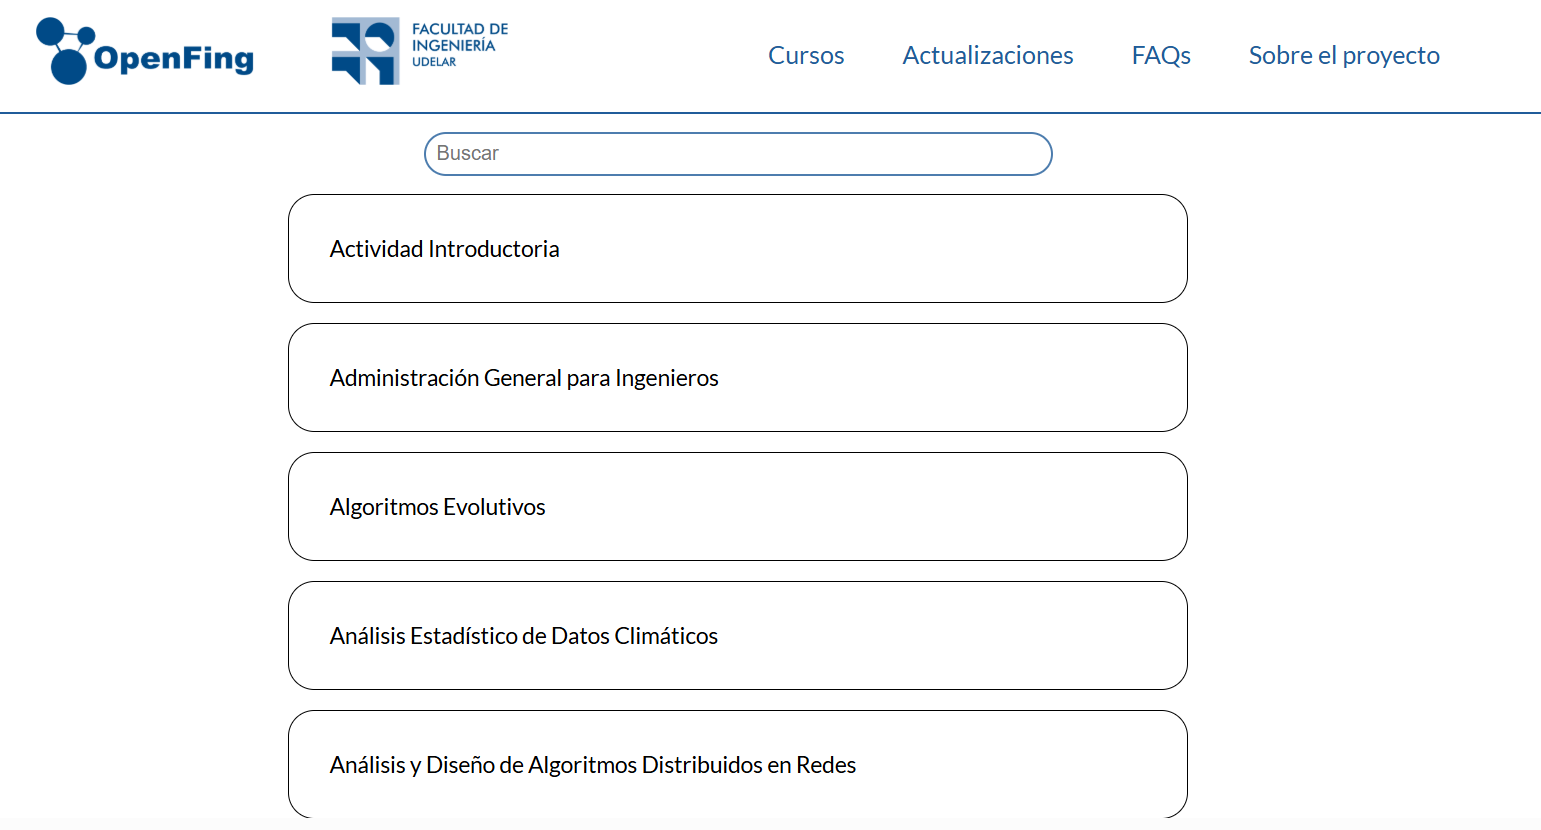
\includegraphics[width=0.8\textwidth]{Nuestro/Imagenes/EstimacionesOpenFing/OpenFing_Pantalla_Inicial}
    \caption{Pantalla inicial con todos los cursos a los que se accedió \protect\footnote{\url{https://open.fing.edu.uy/}}.}
    \label{fig:estimaciones-pantalla-inicial}
\end{figure}

El \textit{scraping} de OpenFing permitió relevar estas clases con el objetivo de estimar el peso total de los videos y la cantidad total de clases.

\subsection{Proceso de transcripción}
\label{subsection:Proceso de transcripción}
\label{Proceso de transcripción}
Para transcribir los videos, primero se los convierte a m4a, solo audio. Este formato es más ligero y no implica pérdida de calidad. Además, la conversión del video a audio sumada al tiempo de transcripción del audio es bastante menor que transcribir el video directamente. Cada transcripción se realiza bajo un modelo determinado; los modelos que transcriben mejor suelen ser más pesados y más lentos.

Para esto se utilizan las bibliotecas ffmpeg, para las conversiones, y faster-whisper, para las transcripciones. Para el proyecto son de valor las marcas de tiempo (\textit{timestamps}) que ofrece Whisper, ya que hay casos de uso que las utilizan. Se obtiene un archivo \acrshort{json} que indica cuándo empieza y termina cada frase.

\subsection{Añadir a una base de datos vectorial}
\label{subsection:Añadir a una base de datos vectorial}
\label{Añadir a una base de datos vectorial}
Este proceso aún puede cambiar según cómo se experimente en la búsqueda de mejores resultados. Involucra la separación de las transcripciones en fragmentos (\textit{chunks}), que pueden ser frases de la transcripción, conjuntos de oraciones o cortes por cantidad de palabras (por ejemplo $\approx 400$), entre otras opciones; la vectorización de esos fragmentos; y el guardado de los vectores en una base vectorial.

También se conservan las marcas de tiempo mencionadas antes, de modo que cada fragmento tenga las suyas, y cada \gls{chunk} incluye los metadatos de la clase asociada.

Para esto se utiliza LangChain.

\subsection[Estimaciones de lo que significaría para OpenFing]{Estimaciones de lo que significaría para OpenFing}
\label{Estimaciones de lo que significaría para OpenFing}
Por último, se tomó una muestra de OpenFing y se le aplicaron los procesos descriptos, con el objetivo de estimar cuánto tiempo y espacio se necesitarían para ejecutarlos sobre la totalidad de OpenFing.

\section{Resultados}
\label{section:Resultados}
\label{Resultados}
Se estima que OpenFing tiene un total aproximado de 1~TB de videos, contabilizando solo los que se encontraron públicos, y 2835 videos públicos en total. A partir de una muestra de transcripciones y conversiones se estimó lo que significaría aplicar todo el proceso al material completo. El tamaño total relevado es de 999,29~GB.

\subsection{Conversiones de mp4 a m4a}
\label{subsection:Conversiones de mp4 a m4a.}
\label{Conversiones de mp4 a m4a.}
Los archivos m4a pueden eliminarse una vez realizadas las transcripciones. Se estima que todos los m4a de los videos pesarían entre 184 y 200~GB; el rango surge de convertir una pequeña cantidad de videos. Se pueden convertir aproximadamente 129,90 horas de video por cada hora de conversión.

\subsection{Velocidad de las transcripciones}
\label{subsection:Velocidad de las Trancripciones}
\label{Velocidad de las Trancripciones}
Los tiempos que se presentan provienen de transcribir con un equipo con las siguientes características.

\begin{itemize}
    \item[\textbf{Hardware:}]
    \begin{itemize}
        \item GPU: NVIDIA GeForce RTX 4050 (6 GB VRAM)
        \item Controlador: NVIDIA 535.247.01
        \item CUDA: versión 12.2
    \end{itemize}
    \item[\textbf{Software:}]
    \begin{itemize}
        \item Modelo ASR: Whisper (OpenAI)
        \item Implementación: faster-whisper 1.1.0
        \item Tamaño de modelo: medium
        \item Idioma: español (es)
        \item Dispositivo: CUDA
    \end{itemize}
    \item[\textbf{Configuración:}]
    \begin{itemize}
        \item Tarea: transcribe
        \item Filtro VAD: activado
        \item \textit{Word timestamps}: activado
        \item \textit{Initial prompt}:
        \begin{quote}
               ``Esta es una clase de la Facultad de Ingeniería de la Universidad de la República (UDELAR), Uruguay. El contenido incluye terminología técnica de ingeniería, conceptos académicos, algoritmos, programación, matemáticas, física y ciencias de la computación. Se utilizan términos técnicos en español rioplatense y ocasionalmente en inglés. Pueden mencionarse tecnologías, frameworks, lenguajes de programación, conceptos de inteligencia artificial, machine learning, estructuras de datos y algoritmos.''
        \end{quote}
    \end{itemize}
\end{itemize}

Se realizaron 180 transcripciones en 8:49:18. Si se consideran esas 180 clases representativas del total, transcribirlas todas demoraría unas 132,7 horas.

\subsection{Calidad de las transcripciones}
\label{subsection:Calidad de las Transcripciones}
\label{Calidad de las Transcripciones}
Para evaluar la calidad se realizaron transcripciones manuales y se compararon con las producidas por los modelos.

Existen estadísticas que indican de forma objetiva qué tan bueno es un modelo. Sin embargo, esas estadísticas no expresan por sí solas la calidad de un modelo o de una transcripción, por lo que a continuación se explica cómo se valoraron los resultados.

Las transcripciones que se consideraron buenas son las de los modelos \textit{small} y \textit{medium}, entre los que no se encontró mayor diferencia. Los resultados son buenos cuando el audio es nítido, que es la mayoría de los casos de OpenFing, y algo peores cuando no lo es, aunque igualmente aceptables. Entre los errores observados con estos modelos está la confusión entre dos palabras similares, a veces con significados parecidos o que son variantes de una misma palabra base. También suele haber errores en nombres propios o apellidos. Además, no captan bien las fórmulas y funciones, que transcriben literalmente: por ejemplo, si el docente menciona ``R de x en función de y'', el modelo suele transcribir eso mismo y no ``R(x) en función de y'', que sería preferible.

De todas formas, los modelos detectan palabras en inglés u otros idiomas cuando se utilizan, incluso con la configuración de solo español, y transcriben correctamente aunque el hablante tenga acento. Los números se escriben con cifras y no con letras.

Los modelos \textit{tiny} y \textit{base} presentan errores bastante más frecuentes, que pueden degradar la eficacia del chatbot.

\begin{figure}[htbp]
    \centering
    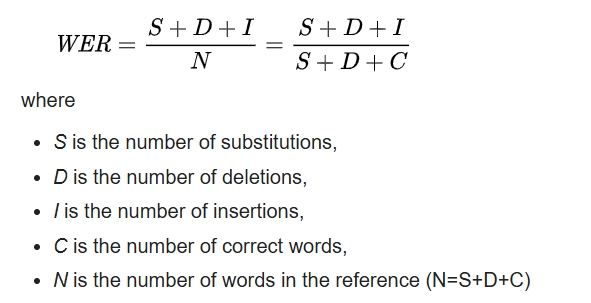
\includegraphics[width=0.8\textwidth]{Nuestro/Imagenes/EstimacionesOpenFing/WordErrorRate.png}
    \caption{Cálculo de la tasa de error de palabras \protect\footnote{\url{https://es.wikipedia.org/wiki/Word_Error_Rate}}.}
    \label{fig:estimaciones-wer}
\end{figure}

\begin{itemize}
    \item \textit{Word Error Rate} (WER): número mínimo de inserciones, borrados y sustituciones de palabras necesarios para transformar una transcripción en la de referencia, dividido por la cantidad de palabras.
    \item MER (\textit{Match Error Rate}): tasa de error general que combina sustituciones, eliminaciones e inserciones. Un valor más bajo indica mayor precisión.
    \item WIL (\textit{Word Information Lost}): mide cuánta información se pierde por errores como sustituciones y eliminaciones. Un valor más bajo indica menos errores críticos.
    \item WIP (\textit{Word Information Preserved}): complemento de WIL, indica cuánta información de la palabra original se preserva. Un valor más alto es mejor.
    \item CER (\textit{Character Error Rate}): porcentaje de caracteres incorrectos respecto del texto de referencia. Un valor más bajo indica mayor precisión.
\end{itemize}

\begin{table}[htbp]
\centering
\caption{Métricas de evaluación de los modelos (ad = autodetección de idioma, es = español).}
\label{tab:estimaciones-metricas}
\begin{tabular}{l l l S[table-format=1.3] S[table-format=1.3] S[table-format=1.3] S[table-format=1.3] S[table-format=1.3]}
\toprule
\textbf{Modelo} & \textbf{Conjunto} & \textbf{Idioma} & \textbf{WER} & \textbf{MER} & \textbf{WIL} & \textbf{WIP} & \textbf{CER} \\
\midrule
medium & clase 1 & ad & 0.046 & 0.045 & 0.071 & 0.928 & 0.023 \\
       &         & es & 0.046 & 0.045 & 0.071 & 0.928 & 0.023 \\
\cmidrule(r){1-8}
medium & clase 2 & ad & 0.086 & 0.085 & 0.120 & 0.879 & 0.052 \\
       &         & es & 0.042 & 0.042 & 0.057 & 0.942 & 0.027 \\
\midrule
small  & clase 1 & ad & 0.150 & 0.148 & 0.248 & 0.751 & 0.054 \\
       &         & es & 0.150 & 0.148 & 0.248 & 0.751 & 0.054 \\
\cmidrule(r){1-8}
small  & clase 2 & ad & 0.139 & 0.137 & 0.219 & 0.780 & 0.059 \\
       &         & es & 0.234 & 0.228 & 0.372 & 0.627 & 0.081 \\
\midrule
base   & clase 1 & ad & 0.203 & 0.199 & 0.324 & 0.675 & 0.076 \\
       &         & es & 0.198 & 0.194 & 0.317 & 0.682 & 0.074 \\
\bottomrule
\end{tabular}
\end{table}
